\documentclass{article}
\usepackage{graphicx,amssymb,amsmath,amsbsy,MnSymbol}

\usepackage[T1]{fontenc}        % pour les charactères accentués
\usepackage[utf8]{inputenc}

\DeclareMathOperator{\score}{score}
\DeclareMathOperator{\tfidf}{tf-idf}


\setlength{\parindent}{0.0in}
\setlength{\parskip}{0.3in}
\setlength{\topmargin}{-0.4in}
\setlength{\topskip}{1in}    % between header and text
\setlength{\textheight}{8in} % height of main text
\setlength{\textwidth}{6in}    % width of text
\setlength{\oddsidemargin}{0.5in} % odd page left margin
\setlength{\evensidemargin}{0.5in} % even page left margin

\bibliographystyle{plain}

\pagenumbering{arabic}
\date{\today}
\title{Smooth object retrieval using Bag of Boundaries}
\author{Vadim Kantorov \& Nelle Varoquaux}
\begin{document}
\maketitle
\begin{abstract}

\end{abstract}

\section{Introduction}
Object recognition is one of the many very active field of vision. Extracting
viewpoints and lightning invariant descriptors is now done efficiently,
allowing performant commercial applications. \\
However, current methods fail on two type of objects: smooth objects and wiry
objects. We will focus on the smooth objects, using methods
\cite{Arandjelovic11} introduces: boundary descriptors. These new descriptors
focus on describing the form of the objects, allowing to retrieve objects
of same shape, but of different sizes and materials. \\
We will use the sculptures 6K dataset: it contains $6000$ pictures of
sculptures, mostly the work of Moore and Rodin, with groundtruth for twenty
of this sculptures. Most sculptures appear several times in the dataset, taken
from different points of views. As Henry Moore often made sculptures of the
same form in different materials, such as bronze and marble, this dataset is
pertinent to test shape and boundaries descriptors.

\section{Segmentation}
\section{Boundary descriptors}

\begin{figure}

\label{boundary-descriptors}
\begin{center}
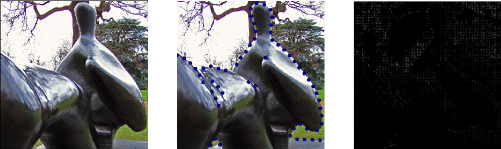
\includegraphics[width=350px]{images/desc.png}
\end{center}
\caption{Boundary descriptors are extracted on a sampled edge, at different
scale. A descriptor is composed of a HoG and a occupancy grid}
\end{figure}

% \caption{The foreground occupancy mask is a grid, where the value of each
% cell represents the ration of foreground pixels.}

\cite{Arandjelovic11} presents a new shape descriptors, invariant to texture
and color, but also lighting, scale and small viewpoints changes. It needs to
be local, in order to be robust to partial occlusions. \\
The boundary descriptors are formed of two descriptors: a Histogram of
Gradients (HoG) and a foreground mask occupancy grid. The first part is a
4 x 4 HoG cells, containing each 8 x 8 pixels, then L2 normalized. The second
part is 4 x 4 occupancy grid, representing the ratio of foreground pixels in
each cell. It is then L1 normalized, and each element is squared root. The two
descriptors are then concatenated, yielding a 340 element descriptor. \\
Each descriptors is computed at three different scales, 1, 4, and 16 times
1/10 of the background at interest points. This are computed  on the sampled
edge, in the manner of \cite{BelongieMP02}, using a minimal distance between
each interest points of 25 pixels.

\section{Retrieval procedure}

Traditional object retrieval procedure represents an image with a bag of
visual words, based on SIFT descriptors. Here, we will use a Bag of Boundary
(BoB) representation developed in \cite{Arandjelovic11}. Descriptors are
rendered indexable by quantizing them. The standard method is to use the
Lloyd's k-means. Unfortunately, that forces one to load all the descriptors in
ram. Extracting the descriptors on the training set yields around 800k
descriptors. \cite{fast-k-means} proposes a much faster, online version of
the k-means, enabling us to compute efficiently the vocabulary on the whole
index. \\
Once the vocabulary is build, the inverse index can be easily build, and fits
in ram, enabling fast retrieval from the database. Results are ranked using
tf-idf. To ensure consistency of the results, a spatial verification is done,
using a very loose affine transformation, implemented using RANSAC (figure
\ref{ransac}). \cite{Arandjelovic11} refines the tf idf scoring using:

\begin{equation*}
\score = \tfidf + \alpha n + \beta \frac{n}{n_q} \frac{n}{n_r}
\end{equation*}

We unfortunately did not have time to implement the reranking.

\begin{figure}
\label{ransac}
\begin{center}
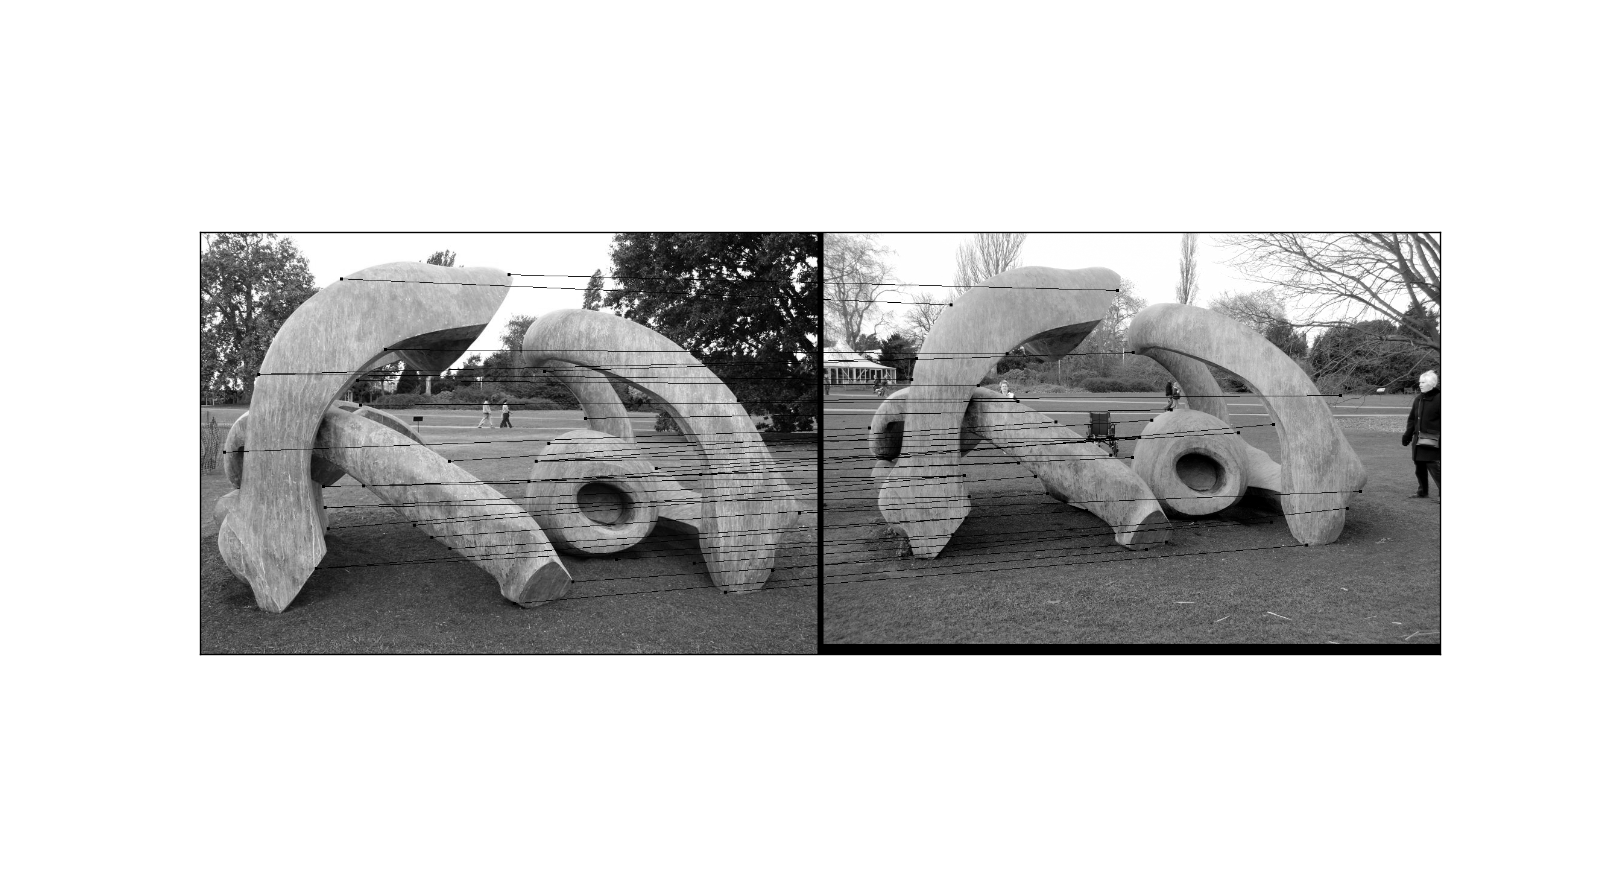
\includegraphics[width=350px]{images/matching_01.png}
\end{center}
\caption{A very loose affine transformation is fitted, using RANSAC}
\end{figure}

\section{Results}

The sculpture 6k dataset is divided into two: a training set, used for
training the segmentation classifier, and a testing set, for everything else.
To test the smooth object retrieval pipeline, 10 sculptures of Henry Moore are
chosen, with seven images for these sculptures. This sums up to 70 queries. \\
For each of these queries, a groundtruth is provided, listing the names of the
\textit{positives} and of \textit{ignores}. The list of \textit{ignores} is
composed of pictures in which less of 25\% of the sculpture is visible.

\section{Conclusion}

\bibliography{biblio.bib}

\end{document}
